\section{Hình thức hoá bài toán tìm kiếm}

Mục này mô tả bài toán theo đúng các thành phần của một bài toán tìm kiếm: trạng thái, hành động, mô hình chuyển trạng thái, kiểm tra đích, hàm chi phí và heuristic. Mục cuối trình bày cách các thuật toán tránh duyệt lại trạng thái. Toàn bộ mô hình nằm trong \texttt{bloxorz/core} và được mọi thuật toán dùng chung.

\subsection{Màn chơi và định dạng tệp}

Một màn chơi là một lưới ký tự trong tệp JSON, kèm danh sách công tắc. Toạ độ ghi dạng \texttt{[hàng, cột]}, bắt đầu từ 0, hàng 0 ở trên cùng.

{\renewcommand{\arraystretch}{1.25}
\begin{longtable}{|l|l|l|}
\hline
\textbf{Ký tự} & \textbf{Ô} & \textbf{Ghi chú} \\ \hline
\endhead
\hline
\endlastfoot
\texttt{.} & Ô trống (void) & Không có sàn \\ \hline
\texttt{\#} & Sàn &  \\ \hline
\texttt{S} & Sàn, vị trí bắt đầu & Đúng 1 ô; khối bắt đầu ở tư thế đứng \\ \hline
\texttt{G} & Lỗ đích & Đúng 1 ô \\ \hline
\texttt{F} & Ô dễ vỡ &  \\ \hline
\texttt{-} / \texttt{=} & Cầu, đóng / mở lúc đầu &  \\ \hline
\texttt{O} & Công tắc mềm & Cần một mục trong \texttt{switches} \\ \hline
\texttt{X} & Công tắc nặng & Cần một mục trong \texttt{switches} \\ \hline
\texttt{T} & Công tắc tách & Cần một mục trong \texttt{switches} \\
\end{longtable}
}

\begin{Verbatim}[breaklines=true, fontsize=\footnotesize, frame=single]
{
  "name": "Ví dụ",
  "grid": ["S#O-=#", "##X--#", "#T#FFG"],
  "switches": [
    {"pos": [0, 2], "effect": "toggle", "bridges": [[0, 3], [0, 4]]},
    {"pos": [1, 2], "effect": "open",   "bridges": [[1, 3], [1, 4]]},
    {"pos": [2, 1], "targets": [[0, 0], [2, 0]]}
  ]
}
\end{Verbatim}

\begin{itemize}
\item Công tắc mềm và công tắc nặng có \texttt{effect} (\texttt{toggle}: đảo trạng thái, \texttt{open}: mở, \texttt{close}: đóng) và \texttt{bridges} (các ô cầu mà công tắc điều khiển).
\item Công tắc tách có \texttt{targets}: hai ô nơi hai khối lập phương xuất hiện. Hai ô này phải khác nhau, không phải ô trống và không kề cạnh nhau, vì hai khối kề nhau sẽ ghép lại ngay (mục 3.4.3).
\item Bộ đọc màn kiểm tra toàn bộ các ràng buộc trên. Tệp sai định dạng bị từ chối với thông báo lỗi chỉ rõ vị trí.
\end{itemize}

\begin{figure}[!htbp]
\centering
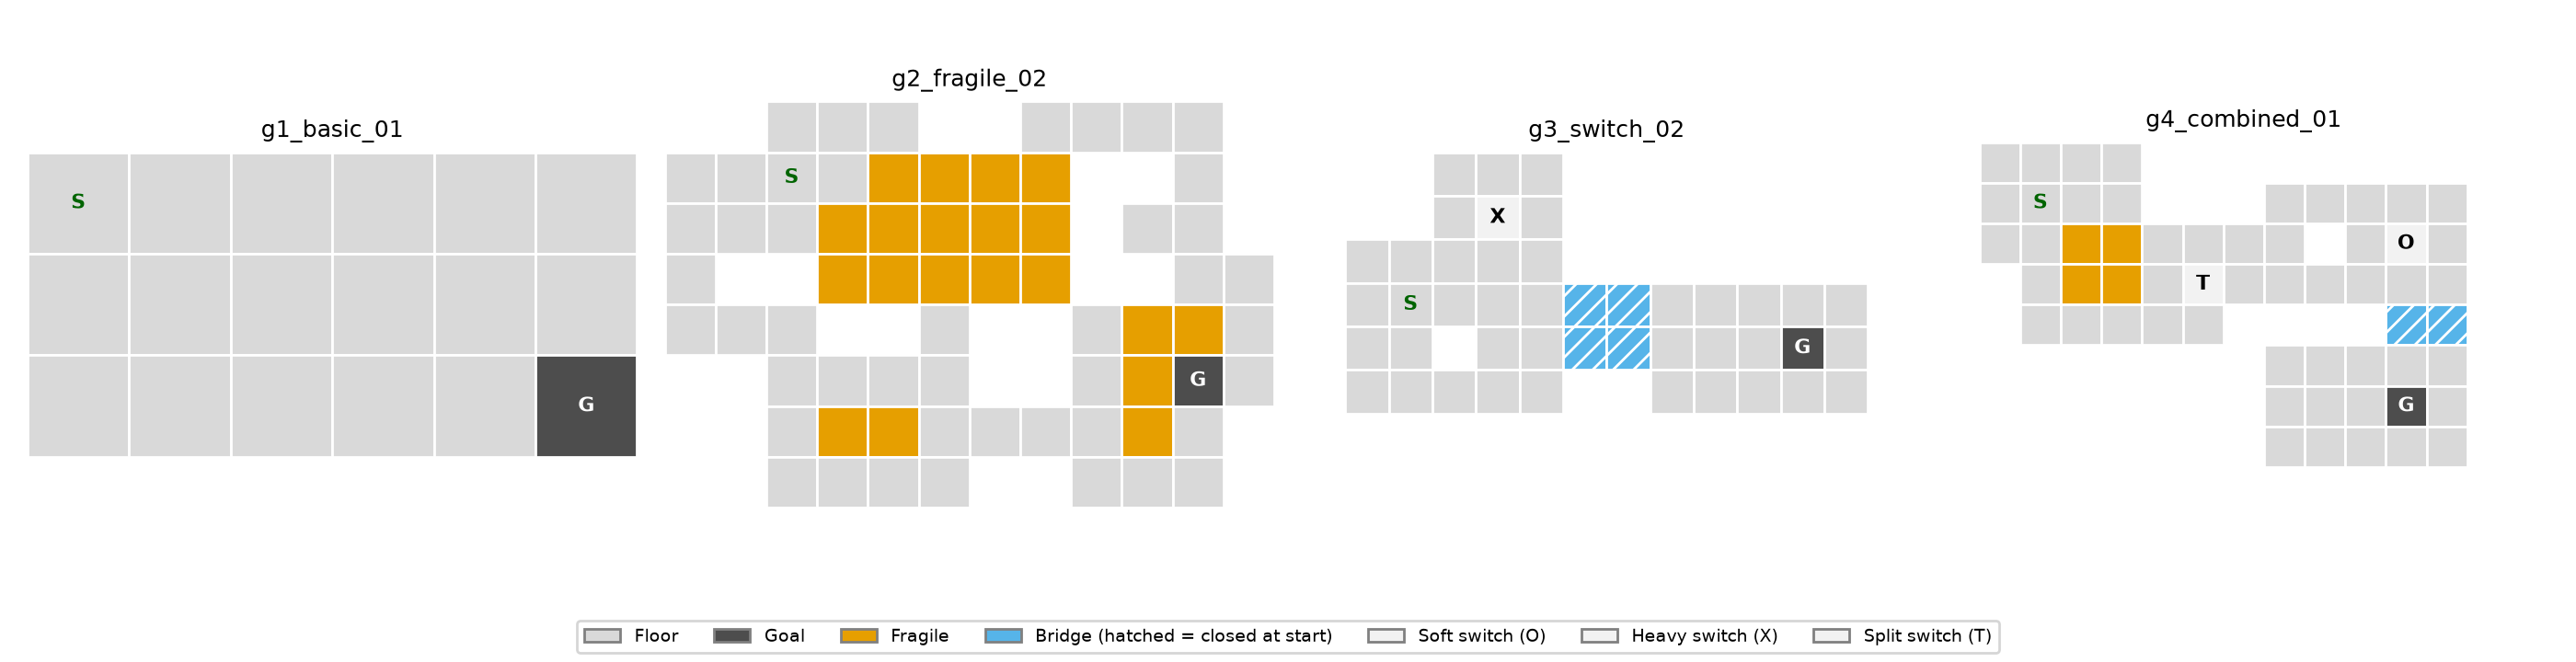
\includegraphics[width=\linewidth,height=0.45\textheight,keepaspectratio]{images/fig_level_groups.png}
\caption{Bốn màn đại diện cho bốn nhóm độ khó (g1: cơ bản; g2: ô dễ vỡ; g3: công tắc và cầu; g4: kết hợp). Ký hiệu S là ô xuất phát, G là ô đích. Các ô cầu gạch chéo ở trạng thái đóng khi bắt đầu.}
\end{figure}

\subsection{Biểu diễn trạng thái}

Phần tĩnh của màn chơi (lưới ô, danh sách công tắc, vị trí đích) nằm trong đối tượng \texttt{Level}. Đối tượng này bất biến và được mọi nút tìm kiếm dùng chung, nên không thuộc trạng thái. Trạng thái chỉ chứa phần thay đổi được, là một \texttt{NamedTuple} \textbf{bất biến và băm được}:

\[s = \langle \text{block}, \text{cubes}, \text{bridges} \rangle\]

{\renewcommand{\arraystretch}{1.25}
\begin{longtable}{|>{\raggedright\arraybackslash}p{0.143\linewidth}|>{\raggedright\arraybackslash}p{0.787\linewidth}|}
\hline
\textbf{Thành phần} & \textbf{Ý nghĩa} \\ \hline
\endhead
\hline
\endlastfoot
\texttt{block} & Khi khối còn nguyên: \texttt{Block(row, col, orientation)} với tư thế \texttt{STANDING}, \texttt{HORIZONTAL} hoặc \texttt{VERTICAL}. Bằng \texttt{None} khi khối đã tách. \\ \hline
\texttt{cubes} & Khi đã tách: \texttt{((r₁, c₁), (r₂, c₂))}, \textbf{phần tử đầu là khối đang được điều khiển}. Bằng \texttt{None} khi khối còn nguyên. \\ \hline
\texttt{bridges} & Số nguyên dùng làm mặt nạ bit: bit thứ \emph{i} bằng 1 nghĩa là ô cầu thứ \emph{i} đang mở. \\
\end{longtable}
}

\begin{itemize}
\item \textbf{Ô neo.} \texttt{Block} được neo ở ô trên cùng bên trái. Tư thế đứng chiếm ô (r, c); nằm ngang chiếm (r, c) và (r, c+1); nằm dọc chiếm (r, c) và (r+1, c).
\item \textbf{Cấu hình cầu thuộc trạng thái.} Hai trạng thái có cùng vị trí khối nhưng khác trạng thái đóng/mở của cầu là \textbf{hai trạng thái khác nhau}, vì khả năng đi tiếp của chúng khác nhau. Đề yêu cầu điều này (mục 3.1 của đề).
\item \textbf{Khối đang điều khiển thuộc trạng thái.} Khi đã tách, \texttt{((a, b), (b, a))} hoán vị là hai trạng thái khác nhau, vì nước đi tiếp theo di chuyển khối khác nhau.
\item \textbf{Mặt nạ bit thay cho tập hợp.} Một số nguyên vừa gọn bộ nhớ, vừa cho phép đóng, mở hay đảo nhiều cầu cùng lúc bằng một phép toán bit (mục 3.4.3).
\end{itemize}

\textbf{Kích thước không gian trạng thái.} Với lưới R×C và m ô cầu, số trạng thái nhiều nhất là 3·R·C·2$^{m}$ (khối nguyên) cộng (R·C)²·2$^{m}$ (khối đã tách). Không gian hữu hạn là cơ sở để chứng minh các thuật toán ở mục 4 và 5 luôn dừng. Trong thực tế số trạng thái đạt tới được nhỏ hơn nhiều: màn lớn nhất (\texttt{g4\_\allowbreak{}combined\_\allowbreak{}04}) có 13 889 trạng thái đạt tới được.

\subsection{Hành động}

Tập hành động là \textbf{Lên (U), Xuống (D), Trái (L), Phải (R)}, cộng thêm \textbf{đổi khối (S)} khi khối đang tách. Các hành động luôn được liệt kê theo \textbf{thứ tự cố định U, D, L, R, (S)}, nên mọi lần chạy cho cùng một kết quả và các thí nghiệm tái lập được. Mỗi trạng thái vì vậy có tối đa 4 nước đi khi khối còn nguyên và tối đa 5 khi đã tách.

\subsection{Mô hình chuyển trạng thái}

Hàm \texttt{result(s, a)} trả về trạng thái kế tiếp, hoặc \texttt{None} nếu nước đi làm khối rơi. Hàm thực hiện bốn bước:

\begin{enumerate}
\item Nếu \texttt{a} là đổi khối S: hoán đổi hai phần tử của \texttt{cubes} và trả về ngay. Vị trí không đổi nên không ô nào phản ứng.
\item Tính vị trí mới: khối nguyên lăn theo bảng chuyển tư thế (mục 3.4.1); khối đã tách thì chỉ khối đang điều khiển đi một ô.
\item Kiểm tra vị trí mới có hợp lệ không (mục 3.4.2). Nếu không, trả về \texttt{None}.
\item Áp dụng hiệu ứng của các ô dưới khối (mục 3.4.3). Bước này có thể đổi cấu hình cầu, tách khối, ghép khối, hoặc làm khối rơi.
\end{enumerate}

\subsubsection{Bảng chuyển tư thế}

Mỗi cặp (tư thế, hướng) ánh xạ xác định tới một cặp (tư thế mới, ô neo mới):

{\small\renewcommand{\arraystretch}{1.25}
\begin{longtable}{|l|l|l|l|l|}
\hline
\textbf{Tư thế \textbackslash{} Hướng} & \textbf{Lên} & \textbf{Xuống} & \textbf{Trái} & \textbf{Phải} \\ \hline
\endhead
\hline
\endlastfoot
Đứng (r, c) & Dọc (r−2, c) & Dọc (r+1, c) & Ngang (r, c−2) & Ngang (r, c+1) \\ \hline
Ngang (r, c) & Ngang (r−1, c) & Ngang (r+1, c) & Đứng (r, c−1) & Đứng (r, c+2) \\ \hline
Dọc (r, c) & Đứng (r−1, c) & Đứng (r+2, c) & Dọc (r, c−1) & Dọc (r, c+1) \\
\end{longtable}
}

\begin{sodo}[!htbp]
\centering
\caption{Chuyển tư thế của khối khi lăn}
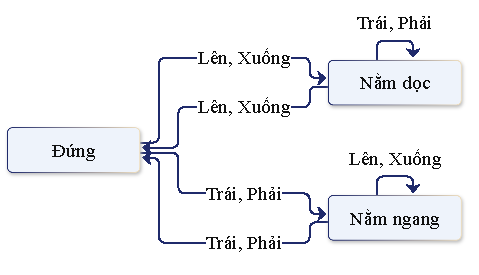
\includegraphics[width=0.62\linewidth,height=0.3\textheight,keepaspectratio]{images/sodo2.pdf}
\end{sodo}

Khối đứng lăn thì ngã thành nằm theo hướng lăn; khối nằm lăn dọc theo trục dài thì dựng lên đứng; khối nằm lăn ngang qua trục dài thì vẫn nằm. Cả 12 ô của bảng đều có test riêng.

\subsubsection{Tính hợp lệ của nước đi}

Một vị trí là hợp lệ khi thoả \textbf{mọi} điều kiện sau:

\begin{itemize}
\item mọi ô khối chiếm đều nằm trong lưới, không phải ô trống và không phải cầu đang đóng (cầu đóng được coi như ô trống);
\item khối nguyên \textbf{đang đứng} thì không nằm trên ô dễ vỡ (toàn bộ trọng lượng dồn vào một ô làm ô vỡ);
\item khi đã tách, hai khối lập phương không trùng ô.
\end{itemize}

Khối nằm (trọng lượng chia cho hai ô) và khối lập phương đơn (nửa trọng lượng) được phép nằm trên ô dễ vỡ.

\subsubsection{Hiệu ứng của ô đặc biệt}

Sau một nước đi hợp lệ, các công tắc dưới khối được kích hoạt theo quy tắc:

{\renewcommand{\arraystretch}{1.25}
\begin{longtable}{|>{\raggedright\arraybackslash}p{0.095\linewidth}|>{\raggedright\arraybackslash}p{0.400\linewidth}|>{\raggedright\arraybackslash}p{0.400\linewidth}|}
\hline
\textbf{Loại công tắc} & \textbf{Điều kiện kích hoạt} & \textbf{Hiệu ứng} \\ \hline
\endhead
\hline
\endlastfoot
Mềm (\texttt{O}) & Bất kỳ phần nào của khối đè lên: đứng, nằm, hoặc một khối lập phương & Đóng, mở hoặc đảo các cầu liên kết \\ \hline
Nặng (\texttt{X}) & Chỉ khối nguyên đứng thẳng trên ô & Đóng, mở hoặc đảo các cầu liên kết \\ \hline
Tách (\texttt{T}) & Chỉ khối nguyên đứng thẳng trên ô & Khối biến mất, hai khối lập phương xuất hiện tại \texttt{targets}; khối tại \texttt{targets[0]} được điều khiển trước \\
\end{longtable}
}

\begin{itemize}
\item \textbf{Cập nhật cầu bằng phép toán bit.} Mỗi công tắc lưu sẵn một mặt nạ M gồm các bit của những cầu nó điều khiển. Đảo trạng thái là \texttt{B \textasciicircum{} M}, mở là \texttt{B \textbar{} M}, đóng là \texttt{B \& \textasciitilde{}M}, với B là \texttt{bridges}.
\item \textbf{Cầu đóng dưới chân khối.} Nếu một công tắc đóng đúng cây cầu khối đang nằm lên, khối mất chỗ đỡ và rơi: nước đi trả về \texttt{None}.
\item \textbf{Chế độ tách.} Mỗi nước đi chỉ di chuyển khối đang điều khiển, một ô một lần. Khối lập phương không kích hoạt được công tắc nặng hay công tắc tách, và không thắng được khi đứng trên đích. Khi đang tách, \textbf{chỉ khối vừa di chuyển} mới kích hoạt công tắc dưới chân nó. Khối đứng yên không kích hoạt lại công tắc nó đang đứng.
\item \textbf{Ghép khối.} Sau mỗi nước đi của một khối lập phương, nếu hai khối kề cạnh nhau (khoảng cách Manhattan bằng 1) thì chúng \textbf{tự ghép ngay} thành một khối nằm: cùng hàng thì thành khối nằm ngang, cùng cột thì thành khối nằm dọc. Hai khối kề chéo không ghép. Vì ghép xảy ra ngay khi vừa kề nhau, ngay trước mọi bước ghép hai khối luôn cách nhau 2 ô.
\end{itemize}

\subsubsection{Các trường hợp biên đã thống nhất}

Đề không quy định một số tình huống. Nhóm thống nhất cách xử lý như sau:

{\renewcommand{\arraystretch}{1.25}
\begin{longtable}{|>{\centering\arraybackslash}p{0.068\linewidth}|>{\raggedright\arraybackslash}p{0.414\linewidth}|>{\raggedright\arraybackslash}p{0.414\linewidth}|}
\hline
\textbf{Mã} & \textbf{Tình huống} & \textbf{Cách xử lý} \\ \hline
\endhead
\hline
\endlastfoot
EC-01 & Công tắc đóng chính cây cầu khối đang nằm lên & Khối mất chỗ đỡ, rơi xuống (thua) \\ \hline
EC-02 & Khối lập phương đứng yên trên công tắc khi khối kia di chuyển & Không kích hoạt lại công tắc dưới khối đứng yên \\ \hline
EC-03 & Hành động đổi khối S & Không di chuyển, không kích hoạt công tắc, giữ nguyên cầu \\ \hline
EC-04 & Ghép khối khi một khối đang đứng trên công tắc mềm & Công tắc không bị kích hoạt lại, vì khối đó không di chuyển \\ \hline
EC-05 & Hai khối lập phương đi vào cùng một ô & Nước đi không hợp lệ (thực tế không xảy ra, vì hai khối đã ghép từ khi kề nhau) \\ \hline
EC-06 & Một trong hai khối lập phương rơi & Thua ngay \\ \hline
EC-07 & Khối nằm đè cùng lúc lên hai công tắc mềm & Kích hoạt lần lượt cả hai; nếu cùng đảo một cầu thì cầu đảo hai lần \\ \hline
EC-08 & Ghép khối ngay trên ô dễ vỡ & An toàn, vì khối sau khi ghép luôn ở tư thế nằm \\ \hline
EC-09 & Vị trí xuất hiện sau khi tách là một công tắc mềm & Công tắc mềm đó được kích hoạt ngay \\ \hline
EC-10 & Vị trí xuất hiện sau khi tách là ô trống hoặc cầu đóng & Khối lập phương rơi (thua) \\
\end{longtable}
}

\subsubsection{Sinh trạng thái kế tiếp}

Hàm \texttt{successors(s)} áp dụng \texttt{result} cho từng hành động theo thứ tự cố định và bỏ các nước đi làm khối rơi (Sơ đồ 3).

\begin{sodo}[!htbp]
\centering
\caption{Sinh các trạng thái kế tiếp \texttt{successors(s)}}
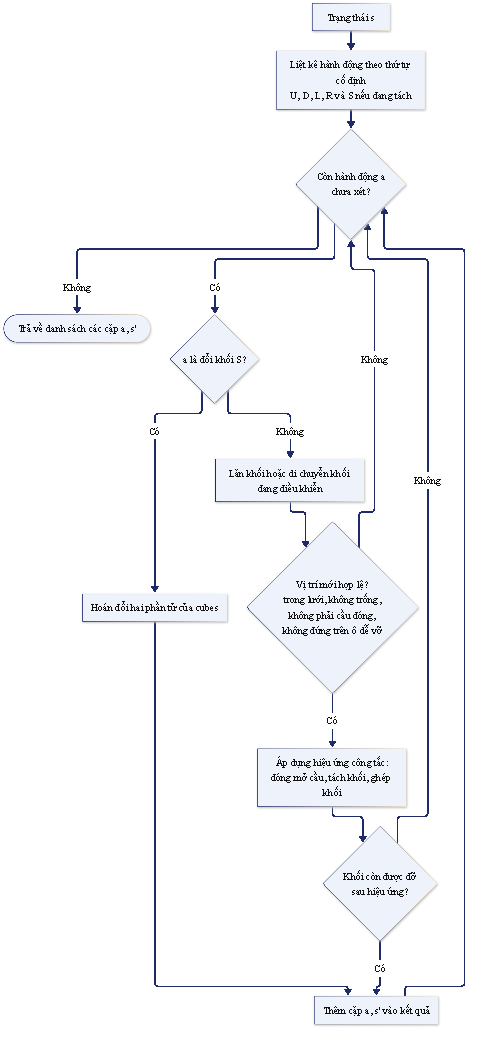
\includegraphics[width=0.95\linewidth,height=0.78\textheight,keepaspectratio]{images/sodo3.pdf}
\end{sodo}

\subsection{Kiểm tra đích}

\texttt{is\_\allowbreak{}goal(s)} đúng khi và chỉ khi khối \textbf{còn nguyên}, ở tư thế \textbf{đứng}, và nằm trên ô đích. Khối nằm vắt qua ô đích hay một khối lập phương đơn trên ô đích đều không thắng.

\subsection{Hàm chi phí}

Nhóm dùng hai hàm chi phí, cùng có dạng \texttt{cost(s, a, s')}:

{\renewcommand{\arraystretch}{1.25}
\begin{longtable}{|>{\raggedright\arraybackslash}p{0.102\linewidth}|>{\raggedright\arraybackslash}p{0.469\linewidth}|>{\raggedright\arraybackslash}p{0.324\linewidth}|}
\hline
\textbf{Hàm} & \textbf{Định nghĩa} & \textbf{Dùng cho} \\ \hline
\endhead
\hline
\endlastfoot
\texttt{unit\_\allowbreak{}cost} & Mọi nước đi tốn 1 & BFS, DFS, IDS (tối ưu theo số nước đi) \\ \hline
\texttt{physics\_\allowbreak{}cost} & Nước đi kết thúc ở tư thế đứng tốn 3, mọi nước đi khác tốn 1 & UCS, A* \\
\end{longtable}
}

\texttt{physics\_\allowbreak{}cost} dựa trên độ nâng trọng tâm của khối khi lăn: dựng khối từ nằm lên đứng phải nâng trọng tâm cao gấp khoảng 3 lần so với một bước lăn ngang. Phần xây dựng và lý giải chi tiết ở mục 5.1.4. Chi phí nhỏ nhất của một bước là 1 với cả hai hàm; heuristic của A* dựa vào tính chất này (mục 5.3).

\subsection{Heuristic}

A* dùng một heuristic ước lượng chi phí còn lại từ khoảng cách Manhattan đến đích chia 2 (một bước lăn đi tối đa 2 ô), xét thêm đường đi qua công tắc tách, và không bao giờ nhỏ hơn chi phí của bước dựng đứng cuối cùng. Công thức và chứng minh tính chấp nhận được, tính nhất quán đối với chính hàm chi phí đã chọn được trình bày ở mục 5.3.

\subsection{Tránh duyệt lại trạng thái}

Do khối có thể lăn qua lại, từ một trạng thái có thể quay về chính nó sau vài nước đi (chẳng hạn lăn sang phải rồi lăn lại sang trái). Đồ thị trạng thái vì vậy có \textbf{chu trình}, và nhiều đường đi khác nhau dẫn tới cùng một trạng thái. Nếu duyệt như duyệt cây, DFS có thể lặp vô hạn còn BFS lãng phí thời gian vào các nhánh trùng lặp. Cả năm thuật toán đều là \textbf{tìm kiếm trên đồ thị}: trạng thái băm được nên dùng trực tiếp làm khoá của \texttt{dict} hoặc phần tử của \texttt{set}, kiểm tra ``đã gặp'' trong thời gian O(1).

{\renewcommand{\arraystretch}{1.25}
\begin{longtable}{|>{\raggedright\arraybackslash}p{0.082\linewidth}|>{\raggedright\arraybackslash}p{0.361\linewidth}|>{\raggedright\arraybackslash}p{0.452\linewidth}|}
\hline
\textbf{Thuật toán} & \textbf{Cấu trúc chống lặp} & \textbf{Quy tắc} \\ \hline
\endhead
\hline
\endlastfoot
BFS & \texttt{parent} (dict) & Trạng thái đã có trong \texttt{parent} thì bỏ qua; mỗi trạng thái vào hàng đợi tối đa một lần \\ \hline
DFS & \texttt{visited} (set) & Đánh dấu khi đưa vào ngăn xếp; mỗi trạng thái vào ngăn xếp tối đa một lần \\ \hline
IDS & \texttt{reached} (dict: trạng thái → độ sâu nhỏ nhất) & Trong mỗi lượt, chỉ đưa lại vào ngăn xếp khi gặp ở độ sâu nhỏ hơn \\ \hline
UCS & \texttt{best\_\allowbreak{}cost} (dict) & Chỉ đẩy vào hàng đợi khi tìm được chi phí nhỏ hơn; bản sao cũ bị bỏ qua khi lấy ra \\ \hline
A* & \texttt{best\_\allowbreak{}g} (dict) & Như UCS; heuristic nhất quán nên mỗi trạng thái được mở rộng tối đa một lần \\
\end{longtable}
}

\subsection{Kiểm thử mô hình}

Mô hình bài toán được kiểm thử tự động bằng \texttt{pytest} (212 test cho toàn bộ dự án):

\begin{itemize}
\item \textbf{Bảng chuyển tư thế:} đủ 12 cặp (tư thế, hướng), và kiểm tra lăn ngược thì về vị trí cũ.
\item \textbf{Bộ đọc màn:} các màn hợp lệ, và từng trường hợp tệp sai định dạng.
\item \textbf{Giao diện bài toán:} rơi khỏi bàn, rơi vào ô trống, thắng và không thắng, thứ tự hành động, đổi khối, phát lại lời giải. Trên màn 1 của trò chơi gốc, lời giải tối ưu 7 nước \texttt{RDDRRDR} đưa khối vào đích, và BFS tìm đúng lời giải này.
\item \textbf{Luật ô đặc biệt (29 test):} ô dễ vỡ và cầu; công tắc mềm và nặng; đóng, mở, đảo cầu và cầu sập dưới chân; công tắc tách; ghép khối; va chạm giữa hai khối lập phương; và một màn có đủ chu trình tách, đổi khối, ghép lại, về đích được BFS giải đúng.
\end{itemize}
